\documentclass[10pt]{beamer}

\usetheme[progressbar=frametitle]{metropolis}
\usepackage{appendixnumberbeamer}

\usepackage{booktabs}
\usepackage[scale=2]{ccicons}

\usepackage{xspace}
\newcommand{\themename}{\textbf{\textsc{metropolis}}\xspace}

\usepackage{verbatim}
\usepackage{physics}
\usepackage{amssymb} % fancy lie algebra letters
\usepackage{tikz}
\newcommand\tikzmark[1]{\tikz[remember picture,overlay]\coordinate (#1);}
\newcommand{\eqname}[1]{\tag*{#1}}% Tag equation with name
\usepackage[absolute]{textpos}
\usepackage{feynmf} % for feynman diagrams
\usepackage{array} % vertically centered table cells
\usepackage{slashed} % slash notation

%Path relative to the main .tex file 
\graphicspath{ {./img/} }

\title{Computational Methods in QFT}
\subtitle{Berends-Giele Recursion}
%\date{\today}
\author{Roman Gruber}
\institute{}
% \titlegraphic{\hfill\includegraphics[height=1.5cm]{logo.pdf}}

\begin{document}

\nocite{*}

\maketitle

\begin{comment}
Notes for the slides

==Motivation==
* Explain the Lagrangian
    * psi = quark field in fundamental repr of SU(3) gauge group
    * gamma^mu Dirac matrices
    * D_mu gauge covariant derivative
    * T_a = genertator of gauge group SU(3) (traceless complex n x n hermitian matrices in the fundamental repr)
    * f^abc structure constants of SU(3), real (conjugate eq [Ta,Tb]=f^^abc...) and antisymmetric (can be seen in eq [2]) in all indices    * a = color index 1-8
    * G = gauge invariant gluon field strength tensor (em field stength tensor F)
    * A^a 8 gluon fields in adjoint repr of SU(3) gauge group
    * m = quark mass
    * g = quark gluon coupling constant
* 1st term in D: quark propagator
* 2nd term in D: quark-gluon vertex
* 3rd term in G: responsible for 3,4-gluon self-interactions

==> From Lagrangian we get (after gauge fixing) Feynman rules of perturbative QCD (see later slide)

==QCD Feynman Rules==
* gauge fixing is Feynman gauge
** R_xi gauge with xi=1:
** -1/(2\xi) ( \partial_{\mu} A^{\mu} )^2
* Just note that we have lots of color dependence with f^abc's
* remove the relations among color factors -> replace all structure constants f^abc with generators T^a

==Color Ordering==
Decomposition of amplitudes -> carry out color part
QCD gauge group: SU(N_c), N_c = 3
dim = N_c^2-1 = 8

* T_a = genertator of gauge group SU(3) (traceless complex n x n hermitian matrices in the fundamental repr)
* f^abc structure constants of SU(3), real (conjugate eq [Ta,Tb]=f^^abc...) and antisymmetric (can be seen in eq [2]) in all indices

* su(N_c) T^a's complete set of traceless herm N_c x N_c matrices (for example the Gell-Mann matrices)
  ** sum over a, a goes from 1 to 8
  ** (1) is the statement that the T^a together with identity form a basis of N times N herm. matrices

* normalization -> avoid sqrt{2}'s in partial amps later
* BLACKBOARD: f^abc = ...
  ** multiply by -i/sqrt(2)
  ** multiply both sides by T^c
  ** Take the trace on both sides Tr(T^c T^c) = 1, for all other T^c's Tr()=0 according to normalisation
  ** BLACKBOARD: derive Fierz identity: see notes

BLACKBOARD: write down Feynman diags: See notes
BLACKBOARD: show color decomp with an example of a 4-gluon scattering
* 4-vertex: look at Feynman rules -> 3 terms with each of them 2 f^abc's -> 2 3-vertices

==Color decopmposition==
n-gluon scattering / tree amplitude
Explain formula:
    fancy A = total / full amplitude
    p_i = 4-momenta, lightlike/massless
    h_i = helicities
    a_i = colors
    g = coupling constant, why n-2 => look at feynman rules
    S_n = Symmetric group, set of all perumtations of n objects
    Z_n = cyclic group, subset of cyclic permutations -> leave trace invariant
    S_N/Z_n = sweep out all distinct cyclic oderings
    A = partial amplitude -> color ordered: they only receive contributions from diagrams with a particular cyclic ordering of the gluons (the order is unimportant as long as its the same for all partial amps)
partial amplitude = color ordered amplitude = dual amplitudes = primitive amplitude (in tree level, not loop level)
for partial amps -> Feynman rules are simplified (without color)

* Fixed ordering of external legs
* Feynman rules are independant of color -> because color part is carried out in the traces
* Singularities and poles can only occure in adjacent momenta -> why?
* We could also use S_{n-1} and fix the first argument and only permute the rest (eq 2.8 in 1507.00332)
* For example if n=5, we have 5!-5=115 terms in the sum. Still alot of terms, but parity (rever
se all helicities), chage conj (exchange q with anti q)

==QCD Feynman rules (color ordered)==
* Because we have stripped all the color factors out of the partial amplitudes, the color-ordered Feynman rules for constructing these objects are purely kinematic (no T^a’s or f^abc’s are left).
* Rules are in Feynman gauge
* To get partial Amplitudes:
  1. draw all color ordered Feynman graphs
  2. evaluate using color ordered Feynman rules
  3. full amp: sum according to eq:decomp

------------spinor helicity-------------------

==Spinor helicity formalism - motivation==
* what are the right kinematic variables for scattering amplitudes?
 * 4-momenta, specially their lorentz-invariant products s_ij
 * Spin? there's a better choice
* label by 4-momentum
* where u_pm(p) are right- and left-handded spinors written in 4-component Dirac notation
* for massless vectors -> 2d, Weyl spinors
* |i> is a column vector 4-comp dirac spinor 
* lambda 2-component version of right-handed spinor
* Negative energy solution v_\pm, but with p^2=0 they are not distinct from u_\pm
* dotted and undotted indices correspond to two different spinor representation of the Lorentz group
* Now we can write the Dirac eq, like this
* build Lorentz-invariant quantities out of these spinors
 * epsilons: antisymmetric tensors

==Spinor helicity formalism - identitites==
* They are for later
* I will mention them again, when I use them in proofs
* recover back our 4-momentum
* Polarization vectors: q is a auxiliary reference momentum, massless q^2=0
 * freedom of on-shell gauge transformation, choice of q is a gauge choice, q not~ p
 * will not motivate this, but epsilons satisfy the following (without proofing them)
  * transverse to momentum p => eps*p = 0
  * e^+ \times (e^+)* = -1
  * e+ \times (e^-)* = 0
  * independent of the helicity of q
  * e+- produce helicity +-1 states

--------BG recursion------------

==The Problem==
* goal to calculate PARTIAL amplitude with first 2 helicities negative, rest positive at tree level, pure gluonic
* first speculated by Parke & Taylor, numerically proven up to n=6
* first proven by Berends & Giele

==Recursion Idea 1/2==
* 1,2,...,n represent a single gluon, with momentum p_i, helicity h_i, but no color a_i -> color eliminated from partial amp
* off-shell current = sum of color-ordered (n+1)-point Feynman graphs, where legs 1,2,...,n are on-shell gluons, and leg “μ” is off-shell
  ** that why the off-shell if mu propagator is included in the current J
  ** mu could also be a quark
  ** gauge dependent <-> depends on reference momenta <-> off-shell quantity

==Recursion Idea 2/2==
* follow the off-shell leg mu into the diagram
  * hit either a 3- or a 4-gluon vertex 
* BLACKBOARD: end of recursion: write down J^{\mu}(i^{\pm}) = \varepsilon ...
* V_3, V_4 are the color ordered Feynman rules, maybe write them down
* BLACKBOARD: write down formula from figure for J^{\mu}


==The Amplitude==
* Amps with n+1 legs are obtained by
  * take J^mu(1,...,n)
  * cut of the off-shell propagator -> multiply by P_{1,n}^2
  * contract with Lorentz index \mu of on-shell polarization vector \eps
  * taking the limit P_{1,n}^2 = p_{n+1}^2 --> 0
* LSZ

==Special case 1==
* all ref momenta are equal
(I will only proof this if I have some time left in the end)

==Special case 2==
* So the reference momenta for the gluons with same helicities are equal.
(I will only proof this if I have some time left in the end)
* How did Berends and Giele came up with this?
  * In trying to prove PT, they thought about what currents appear
  * Jppp and Jmppp, then they calculated the n=1,2,3 cases
  * Then made an ansatz/guess for the n-th case
  * Then proof by induction


==Parke Taylor Formula==
BLACKBOARD: prove A_{n+1}^{tree}(1^{-}, 2^{+}, \dots, n^{+}, (n+1)^{-})

\end{comment}

\begin{frame}{Table of contents}
  \setbeamertemplate{section in toc}[sections numbered]
  \tableofcontents[hideallsubsections]
\end{frame}

\section{Color Ordering}

\begin{frame}[fragile]{Motivation}

    \begin{itemize}[<+->]
        \item Only deal with kinematic variables
        \item Not obstructed by colors
        \item Divide and conquer
        \item QCD Lagrangian \cite{eidemueller2000}:
            \begin{align*}
                L = \bar{\psi} &\left( i \gamma^{\mu} D_{\mu} - m \right) \psi - \frac{1}{4} G^{a}_{\mu \nu} G_{a}^{\mu \nu} \\
                G^{a}_{\mu \nu} &= \partial_{\mu} A^a_{\nu} - \partial_{\nu}A^a_{\mu} + g f^{abc}A^b_{\mu} A^c_{\nu} \\
                D_{\mu} &= \partial_{\mu} - ig T_a A^a_{\mu}
            \end{align*}
    \end{itemize}

\end{frame}

\begin{frame}{QCD Feynman rules \cite{mangano99}}

{\scriptsize
\begin{align*}
    \begin{gathered}
        \begin{fmffile}{diagram_3gluon_vertex}
        \fmfframe(0,10)(0,10){
        \begin{fmfgraph*}(30,30)
            \fmfstraight
            \fmfset{arrow_len}{2mm}
            \fmfset{curly_len}{2mm}
            \fmfset{thin}{0.8pt}
            \fmfpen{thin}
            \fmfleft{g1}
            \fmfright{g2,g3}
            \fmf{gluon}{g1,v}
            \fmflabel{$k,a,\mu$}{g1}
            \fmf{gluon}{g3,v}
            \fmflabel{$p,b,\nu$}{g3}
            \fmf{gluon}{g2,v}
            \fmflabel{$q,c,\rho$}{g2}
        \end{fmfgraph*}
        }
        \end{fmffile}
    \end{gathered}
    &= \frac{i g}{\sqrt{2}} f^{abc} \left[ \eta^{\nu \rho} (p-q)^{\mu} + \eta^{\rho \mu} (q-k)^{\nu} + \eta^{\mu \nu} (k-p)^{\rho} \right], \\
    \begin{gathered}
        \begin{fmffile}{diagram_4gluon_vertex}
        \fmfframe(0,10)(0,10){
        \begin{fmfgraph*}(30,30)
            \fmfstraight
            \fmfset{arrow_len}{2mm}
            \fmfset{curly_len}{2mm}
            \fmfset{thin}{0.8pt}
            \fmfpen{thin}
            \fmfleft{i1,i2}
            \fmfright{o1,o2}
            \fmf{gluon}{i1,v}
            \fmflabel{$d,\sigma$}{i1}
            \fmf{gluon}{i2,v}
            \fmflabel{$a,\mu$}{i2}
            \fmf{gluon}{o2,v}
            \fmflabel{$b,\nu$}{o2}
            \fmf{gluon}{o1,v}
            \fmflabel{$c,\rho$}{o1}
        \end{fmfgraph*}
        }
        \end{fmffile}
    \end{gathered}
    &= -i g^2 \left[
        \begin{array}{l}
            \phantom{+} f^{abe} f^{cde} (\eta^{\mu \rho} \eta^{\nu \sigma} -  \eta^{\mu \sigma} \eta^{\nu \rho}) \\
                     +  f^{ace} f^{bde} (\eta^{\mu \nu}  \eta^{\rho \sigma} - \eta^{\mu \sigma} \eta^{\rho \nu}) \\
                     +  f^{ade} f^{bce} (\eta^{\mu \nu}  \eta^{\sigma \rho} - \eta^{\mu \rho} \eta^{\sigma \nu})
        \end{array}\right], \\
    \begin{gathered}
        \begin{fmffile}{diagram_gluon_fermion_vertex_a}
        \fmfframe(0,10)(15,10){
        \begin{fmfgraph*}(30,30)
            \fmfstraight
            \fmfset{arrow_len}{2mm}
            \fmfset{curly_len}{2mm}
            \fmfset{thin}{0.8pt}
            \fmfpen{thin}
            \fmfright{f1,f2}
            \fmfleft{g1}
            \fmf{gluon}{g1,v}
            \fmflabel{$a,\mu$}{g1}
            \fmf{fermion}{v,f1}
            \fmflabel{$f^{\prime},\bar{\jmath}$}{f1}
            \fmf{fermion}{f2,v}
            \fmflabel{$f,i$}{f2}
        \end{fmfgraph*}
        }
        \end{fmffile}
    \end{gathered}
    &= -\frac{i g \gamma^{\mu} \delta^{f^{\prime}}_{f} }{\sqrt{2}} {(T^a)_i}^{\bar{\jmath}},
    \quad\quad\quad
    \begin{gathered}
        \begin{fmffile}{diagram_gluon_prop}
        \fmfframe(15,10)(15,10){
        \begin{fmfgraph*}(20,25)
            \fmfstraight
            \fmfset{arrow_len}{2mm}
            \fmfset{curly_len}{2mm}
            \fmfset{thin}{0.8pt}
            \fmfpen{thin}
            \fmfright{g1}
            \fmfleft{g2}
            \fmf{gluon,label=$p$}{g2,g1}
            \fmflabel{$a,\mu$}{g2}
            \fmflabel{$b,\nu$}{g1}
        \end{fmfgraph*}
        }
        \end{fmffile}
    \end{gathered}
    = -\frac{i \delta^{ab} \eta^{\mu \nu}}{p^2}, \\
    \begin{gathered}
        \begin{fmffile}{diagram_gluon_fermion_vertex_b}
        \fmfframe(0,10)(15,10){
        \begin{fmfgraph*}(30,30)
            \fmfstraight
            \fmfset{arrow_len}{2mm}
            \fmfset{curly_len}{2mm}
            \fmfset{thin}{0.8pt}
            \fmfpen{thin}
            \fmfleft{f1,f2}
            \fmfright{g1}
            \fmf{gluon}{v,g1}
            \fmflabel{$a,\mu$}{g1}
            \fmf{fermion}{v,f1}
            \fmflabel{$f^{\prime},\bar{\jmath}$}{f1}
            \fmf{fermion}{f2,v}
            \fmflabel{$f,i$}{f2}
        \end{fmfgraph*}
        }
        \end{fmffile}
    \end{gathered}
    &= \frac{i g \gamma^{\mu} \delta^{f^{\prime}}_{f} }{\sqrt{2}} {(T^a)_i}^{\bar{\jmath}},
    \quad\quad\quad
    \begin{gathered}
        \begin{fmffile}{diagram_fermion_prop}
        \fmfframe(15,10)(20,10){
        \begin{fmfgraph*}(20,25)
            \fmfstraight
            \fmfset{arrow_len}{2mm}
            \fmfset{curly_len}{2mm}
            \fmfset{thin}{0.8pt}
            \fmfpen{thin}
            \fmfright{f1}
            \fmfleft{f2}
            \fmf{fermion,label=$p$}{f1,f2}
            \fmflabel{$f,i$}{f2}
            \fmflabel{$f^{\prime},j$}{f1}
        \end{fmfgraph*}
        }
        \end{fmffile}
    \end{gathered}
    = \frac{i \delta^{f^{\prime}}_f \delta^i_j }{p^2}.
\end{align*}
}

\end{frame}

\begin{frame}[fragile]{Color ordering \cite{bg87colorordering}}

    \begin{itemize}[<+->]
    	\item[] QCD gauge group:
    	\begin{itemize}[<+->]
    	    \item $SU(N_c)$ with $N_c=3$
    	    \item $dim(SU(N_c))=N_c^2-1 = 8$
    	\end{itemize}
    	\item[] Lie Algebra:
    	    \begin{itemize}[<+->]
    	    \item $\mathfrak{su}(N_c)$ traceless hermitian with generators ${(T^a)_{i}}^{\bar{\jmath}}$
            \item Fierz identity:

            \begin{align}
                (T^a)_{i_1}^{\bar{\jmath}_1} (T^a)_{i_2}^{\bar{\jmath}_2} = \delta_{i_1}^{\bar{\jmath}_2} \delta_{i_2}^{\bar{\jmath}_1} - \frac{1}{N_c} \delta_{i_1}^{\bar{\jmath}_1} \delta_{i_2}^{\bar{\jmath}_2} \label{eq:fierz}
            \end{align}

    	    \item Normalisation $Tr(T^a T^b) = \delta^{ab}$

    	    \item Structure constants $[T^a, T^b] = i\sqrt{2} \sum_{c=1}^{N_c^2-1} f^{abc} T^c$

            \item[] \begin{align}
                f^{abc} = - \frac{i}{\sqrt{2}} \left( Tr(T^a T^b T^c) - Tr(T^a T^c T^b) \right) \label{eq:fabc}
            \end{align}

    	    \end{itemize}

    \end{itemize}

\end{frame}

{\setbeamercolor{palette primary}{fg=black, bg=black}
\begin{frame}[standout]
    On the blackboard\\
    - Derive the Fierz identity (only if enough time) \\
    - Draw Feynman graphs for the two equations \eqref{eq:fierz} and \eqref{eq:fabc}
\end{frame}
}

{\setbeamercolor{palette primary}{fg=black, bg=black}
\begin{frame}[standout]
    On the blackboard \\
    - Motivate color deomposition with example: 4-gluon scattering
\end{frame}
}

\begin{frame}[fragile]{Color Decopmposition of tree amplitudes}

    \begin{itemize}[<+->]
        \item[] Treat color degrees of freedom by separating them from kinematical parts $\rightarrow$ \alert{partial amplitudes} \cite{bg87colorordering}

        {\scriptsize
        \begin{equation}
            \begin{aligned}
                \mathcal{A}_n^{tree}(\{p_i, &h_i, a_i\}) \\
                = &g^{n-2} \sum_{\sigma \in S_n/Z_n} Tr(T^{a_{\sigma(1)}} \dots T^{a_{\sigma(n)}}) A_n^{tree}(p_{\sigma(1)}, \dots, p_{\sigma(n)}, h_{\sigma(1)}, \dots, h_{\sigma(n)}) \label{eq:decomp}
            \end{aligned}
        \end{equation}
        }

        \begin{itemize}[<+->]
            \item Fixed ordering of external legs
            \item Feynman rules are independant of color
            \item Singularities and poles can only occure in adjacent momenta
        \end{itemize}
    \end{itemize}

\end{frame}

\begin{frame}{Color ordered Feynman rules \cite{johansson2016}}

{\scriptsize
\begin{align*}
    \begin{gathered}
        \begin{fmffile}{diagram_co_3gluon_vertex}
        \fmfframe(0,10)(0,10){
        \begin{fmfgraph*}(30,30)
            \fmfstraight
            \fmfset{arrow_len}{2mm}
            \fmfset{curly_len}{2mm}
            \fmfset{thin}{0.8pt}
            \fmfpen{thin}
            \fmfleft{g1}
            \fmfright{g2,g3}
            \fmf{gluon}{g1,v}
            \fmflabel{$k,\mu$}{g1}
            \fmf{gluon}{g3,v}
            \fmflabel{$p,\nu$}{g3}
            \fmf{gluon}{g2,v}
            \fmflabel{$q,\rho$}{g2}
        \end{fmfgraph*}
        }
        \end{fmffile}
    \end{gathered}
    &= \frac{i}{\sqrt{2}} \left[ \eta^{\nu \rho} (p-q)^{\mu} + \eta^{\rho \mu} (q-k)^{\nu} + \eta^{\mu \nu} (k-p)^{\rho} \right], \\
    \begin{gathered}
        \begin{fmffile}{diagram_co_4gluon_vertex}
        \fmfframe(0,10)(0,10){
        \begin{fmfgraph*}(30,30)
            \fmfstraight
            \fmfset{arrow_len}{2mm}
            \fmfset{curly_len}{2mm}
            \fmfset{thin}{0.8pt}
            \fmfpen{thin}
            \fmfleft{i1,i2}
            \fmfright{o1,o2}
            \fmf{gluon}{i1,v}
            \fmflabel{$\sigma$}{i1}
            \fmf{gluon}{i2,v}
            \fmflabel{$\mu$}{i2}
            \fmf{gluon}{o2,v}
            \fmflabel{$\nu$}{o2}
            \fmf{gluon}{o1,v}
            \fmflabel{$\rho$}{o1}
        \end{fmfgraph*}
        }
        \end{fmffile}
    \end{gathered}
    &= \frac{i}{2} \left[ 2\eta^{\mu \rho} \eta^{\nu \sigma} - \eta^{\mu \nu} \eta^{\rho \sigma} - \eta^{\mu \sigma} \eta^{\nu \rho}\right], \\
    \begin{gathered}
        \begin{fmffile}{diagram_co_gluon_fermion_vertex_a}
        \fmfframe(0,10)(15,10){
        \begin{fmfgraph*}(30,30)
            \fmfstraight
            \fmfset{arrow_len}{2mm}
            \fmfset{curly_len}{2mm}
            \fmfset{thin}{0.8pt}
            \fmfpen{thin}
            \fmfright{f1,f2}
            \fmfleft{g1}
            \fmf{gluon}{g1,v}
            \fmflabel{$\mu$}{g1}
            \fmf{fermion}{v,f1}
            \fmflabel{$f^{\prime}$}{f1}
            \fmf{fermion}{f2,v}
            \fmflabel{$f$}{f2}
        \end{fmfgraph*}
        }
        \end{fmffile}
    \end{gathered}
    &= -\frac{i \gamma^{\mu} \delta^{f^{\prime}}_{f} }{\sqrt{2}},
    \quad\quad\quad
    \begin{gathered}
        \begin{fmffile}{diagram_co_gluon_prop}
        \fmfframe(15,10)(15,10){
        \begin{fmfgraph*}(20,25)
            \fmfstraight
            \fmfset{arrow_len}{2mm}
            \fmfset{curly_len}{2mm}
            \fmfset{thin}{0.8pt}
            \fmfpen{thin}
            \fmfright{g1}
            \fmfleft{g2}
            \fmf{gluon,label=$p$}{g2,g1}
            \fmflabel{$\mu$}{g2}
            \fmflabel{$\nu$}{g1}
        \end{fmfgraph*}
        }
        \end{fmffile}
    \end{gathered}
    = -\frac{i \eta^{\mu \nu}}{p^2}, \\
    \begin{gathered}
        \begin{fmffile}{diagram_co_gluon_fermion_vertex_b}
        \fmfframe(0,10)(15,10){
        \begin{fmfgraph*}(30,30)
            \fmfstraight
            \fmfset{arrow_len}{2mm}
            \fmfset{curly_len}{2mm}
            \fmfset{thin}{0.8pt}
            \fmfpen{thin}
            \fmfleft{f1,f2}
            \fmfright{g1}
            \fmf{gluon}{v,g1}
            \fmflabel{$\mu$}{g1}
            \fmf{fermion}{v,f1}
            \fmflabel{$f^{\prime}$}{f1}
            \fmf{fermion}{f2,v}
            \fmflabel{$f$}{f2}
        \end{fmfgraph*}
        }
        \end{fmffile}
    \end{gathered}
    &= \frac{i \gamma^{\mu} \delta^{f^{\prime}}_{f} }{\sqrt{2}},
    \quad\quad\quad
    \begin{gathered}
        \begin{fmffile}{diagram_co_fermion_prop}
        \fmfframe(15,10)(20,10){
        \begin{fmfgraph*}(20,25)
            \fmfstraight
            \fmfset{arrow_len}{2mm}
            \fmfset{curly_len}{2mm}
            \fmfset{thin}{0.8pt}
            \fmfpen{thin}
            \fmfright{f1}
            \fmfleft{f2}
            \fmf{fermion,label=$p$}{f1,f2}
            \fmflabel{$f$}{f2}
            \fmflabel{$f^{\prime}$}{f1}
        \end{fmfgraph*}
        }
        \end{fmffile}
    \end{gathered}
    = \frac{i \delta^{f^{\prime}}_f }{p^2}.
\end{align*}
}

\end{frame}


\section{Spinor helicity formalism for massless vector bosons}

\begin{frame}{Spinor helicity formalism \cite{dixon2016}, \cite{berends81} - motivation}

    \begin{itemize}[<+->]
        \item[] What are the right kinematic variables for scattering amplitudes?
        \item[] Organize spin quantum numbers for external states
        \item[] $\rightarrow$ \alert{helicity basis} {\scriptsize
        \begin{align*}
            p^{\mu}_i, h_i \rightarrow u_{-}(p_i) &= \begin{pmatrix} \lambda_{i \alpha} \\ 0 \\ 0\end{pmatrix} \leftrightarrow | i \rangle = \lambda_{i \alpha} = \begin{pmatrix}\cdot \\ \cdot\end{pmatrix} \\
            u_{+}(p_i) &= \begin{pmatrix}0 \\ 0 \\ \tilde{\lambda}_{i}^{\dot{\alpha}} \end{pmatrix} \leftrightarrow | i \rbrack = \tilde{\lambda}^{\dot{\alpha}}_i = \begin{pmatrix}\cdot \\ \cdot\end{pmatrix}
        \end{align*}
        }
        \item[] Massless \alert{Dirac equation}: {\scriptsize $\slashed{p}_i | i \rangle = \slashed{p}_i | i \rbrack = 0$ }
        \item[] Define \alert{spinor products}: {\scriptsize
        \begin{align*}
            \langle ij \rangle &\equiv \lambda^{\alpha}_i \epsilon_{\alpha \beta} \lambda^{\beta}_j \\
            \lbrack ij \rbrack &\equiv \tilde{\lambda}_{i \dot{\alpha}} \epsilon^{\dot{\alpha} \dot{\beta}} \tilde{\lambda}_{j \dot{\beta}}
        \end{align*}
        } with {\scriptsize
        \begin{align*}
            \epsilon_{\alpha \beta} &= \begin{pmatrix}0 & -1 \\ 1 & 0\end{pmatrix}, & \epsilon^{\alpha \beta} &= \begin{pmatrix}0 & 1 \\ -1 & 0\end{pmatrix}
        \end{align*}
        }
    \end{itemize}

\end{frame}

\begin{frame}{Spinor helicity formalism - important identities}

    \begin{itemize}[<+->]
        \item Anti-symmetry: {\scriptsize$\langle ij \rangle = - \langle ji \rangle$}, {\scriptsize$\lbrack ij \rbrack = - \lbrack ji \rbrack$}, {\scriptsize$\langle ii \rangle = \lbrack ii \rbrack = 0$}
        \item Squaring: {\scriptsize$\langle ij \rangle \lbrack ji \rbrack = 2 p_i \cdot p_j = \left( p_i + p_j \right)^2 =: s_{ij}$}
        \item 4-momentum: {\scriptsize$p^{\mu} = \frac{1}{2} \langle p | \sigma^{\mu} | p \rbrack $}
        \item Slash: {\scriptsize$\slashed{p} = | p \rangle \lbrack p | + | p \rbrack \langle p |$}
        \item Fierz: {\scriptsize$ \langle i | \sigma^{\mu} | j \rbrack \langle k | \sigma_{\mu} | \ell \rbrack = 2 \langle ik \rangle \lbrack \ell j \rbrack$}
        \item Charge conj.: {\scriptsize$ \langle i | \sigma^{\mu} | j \rbrack = \lbrack j | \overline{\sigma}^{\mu} | i \rangle$}
        \item Shouten: {\scriptsize$ \langle ij \rangle \langle k | + \langle jk \rangle \langle i | + \langle ki \rangle \langle j | = 0$}
        \item Polarization vectors \cite{xu86}: {\scriptsize
        \begin{align*}
            \varepsilon_{+}^{\mu}(p,q) = \frac{1}{\sqrt{2}} \frac{\langle q | \sigma^{\mu} | p \rbrack }{ \langle qp \rangle } \quad \text{and} \quad \varepsilon_{-}^{\mu}(p,q) = - \frac{1}{\sqrt{2}} \frac{\lbrack q | \overline{\sigma}^{\mu} | p \rangle }{ \lbrack qp \rbrack }
        \end{align*}
        }
    \end{itemize}

\end{frame}

\section{Parke-Taylor Formula / Berends-Giele Recursion}

\begin{frame}{The Problem}

\begin{itemize}[<+->]
    \item[] Parke-Taylor Formula:
    \begin{align*}
        A_{n}^{tree}(1^{-}, 2^{-}, 3^{+}, \dots, n^{+}) = i\frac{\langle 12 \rangle^4}{\langle 12 \rangle \dots \langle n1 \rangle}
    \end{align*}

    \item[] "Also, we challenge the string theorists to prove more rigorously that eqn(3) is correct." \cite{pt86}  
    \item[] General Parke-Taylor Formula \cite{bg88recursive}:
    \begin{align*}
        A_{jk}^{tree,MHV} = A_{n}^{tree}(1^{+}, \dots, j^{-}, \dots, k^{-}, \dots, n^{+}) = i\frac{\langle jk \rangle^4}{\langle 12 \rangle \dots \langle n1 \rangle}
    \end{align*}
    \item[] MHV: maximally helicity violating amplitudes
\end{itemize}

\end{frame}

\begin{frame}{Recursion Idea 1/2 \cite{bg88recursive}}

\begin{itemize}[<+->]
    \item[] More external legs $\rightarrow$ more complexity
    \item[] Auxiliary quantity with one off-shell leg $\mu$
    \item[] Off-shell current $J^{\mu}(1, 2, \dots, n)$ $\rightarrow$ sum of all color ordered graphs:
    \item[]
    \begin{align*}
        \begin{gathered}
            \begin{fmffile}{diagram_ngluons}
                \fmfframe(0,0)(10,0){
                \begin{fmfgraph*}(60,60)
                    \fmfkeep{current}
                    \fmfset{arrow_len}{2mm}
                    \fmfset{curly_len}{2mm}
                    \fmfset{thin}{0.8pt}
                    \fmfpen{thin}
                    \fmfsurround{ph1,g2,g1,ph2,gi,ph3,gn,gnm}
                    \fmf{gluon}{gi,v}
                    \fmf{gluon}{v,g1}
                    \fmf{gluon}{v,g2}
                    \fmf{phantom}{v,ph1}
                    \fmf{phantom}{v,ph2}
                    \fmf{phantom}{v,ph3}
                    \fmf{gluon}{v,gnm}
                    \fmf{gluon}{v,gn}
                    \fmflabel{$\mu$}{gi}
                    \fmflabel{$1$}{g1}
                    \fmflabel{$2$}{g2}
                    \fmflabel{$n$}{gn}
                    \fmflabel{$n-1$}{gnm}
                    \fmflabel{$\vdots$}{ph1}
                    \fmfblob{.15w}{v}
                    \fmfv{decoration.shape=circle,decoration.filled=empty,decoration.size=.25w,label=$J^{\mu}$,label.dist=0}{v}
                \end{fmfgraph*}
                }
            \end{fmffile}
        \end{gathered}
    \end{align*}

\end{itemize}

\end{frame}

\begin{frame}{Recursion Idea 2/2 \cite{bg88recursive}}

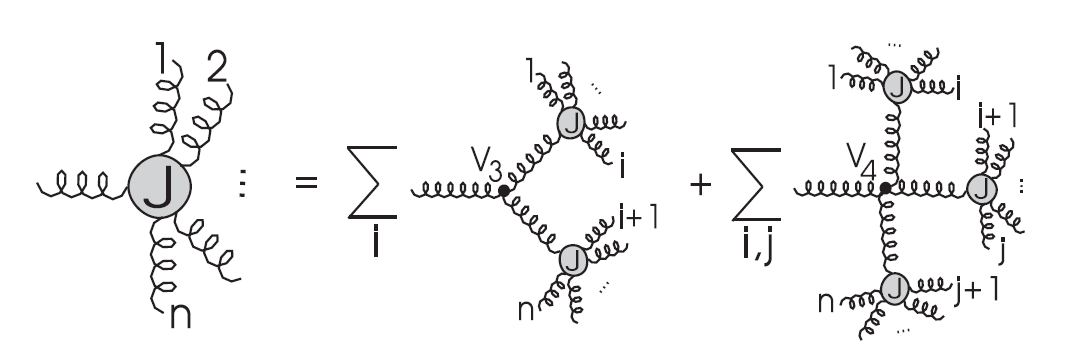
\includegraphics[scale=0.4,natwidth=1079,natheight=359]{rec.png}

\begin{figure}[!h]
\advance\leftskip-4cm
\tikz[baseline=0.6ex] \shade[top color=black, bottom color=black] (0,0) rectangle (16cm,8cm);
\end{figure}

\end{frame}

{\setbeamercolor{palette primary}{fg=black, bg=black}
\begin{frame}[standout]
    On the blackboard\\
    - Write down formula for $J^{\mu}$ (reading it off the picture in the previous slide) \\
    - The $i=1$ case: $J^{\mu}(1^{\pm}) = \varepsilon ...$
\end{frame}
}

\begin{frame}{The Amplitude}

\begin{itemize}[<+->]
    \item[] How to get the \alert{partial} Amplitude? \cite{lsz55}
    \begin{itemize}[<+->]
        \item Take $J^{\mu}(1,2, \dots ,n)$
        \item Cut off the off-shell propagator
        \item Contract with Lorentz index $\mu$ of on-shell polarization vector $\varepsilon$
        \item Take the limit $P_{1,n}^2 = p_{n+1}^2 \to 0$
    \end{itemize}
    \item[] How to get the \alert{full} Amplitude?
    \begin{itemize}[<+->]
        \item Take the partial amplitudes
        \item Dress them with traces
        \item Sum over all different color orderings
        \item[] {\scriptsize
        \begin{equation*}
            \begin{aligned}
                \mathcal{A}_n^{tree}(\{p_i, &h_i, a_i\}) \\
                = &g^{n-2} \sum_{\sigma \in S_n/Z_n} Tr(T^{a_{\sigma(1)}} \dots T^{a_{\sigma(n)}}) A_n^{tree}(p_{\sigma(1)}, \dots, p_{\sigma(n)}, h_{\sigma(1)}, \dots, h_{\sigma(n)})
            \end{aligned}
        \end{equation*}
        }
    \end{itemize}
\end{itemize}

\end{frame}

\begin{frame}{Special case 1/2}

If only the helicity of the first gluon is negative and the rest are positive, then the equation for $J^{\mu}$ reduces to the following form \cite{bg88recursive}:

\begin{align}
    J^{\mu}(1^{-}, 2^{+}, \dots , n^{+}) = \frac{ \bra{1} \sigma^{\mu} \slashed{P}_{2,n} \ket{1} }{ \sqrt{2} \langle 12 \rangle \cdots \langle n1 \rangle } \sum_{m=3}^{n} \frac{ \bra{1} \slashed{p}_m \slashed{P}_{1,m} \ket{1} }{ P_{1,m-1}^2 P_{1,m}^2 },
\end{align}

where the reference momenta are $q_1 = p_2$ and $q_2 = \dots = q_n = p_1$.

\end{frame}

\begin{frame}{Special case 2/2}

If the helicities of all participating gluons are equal, then the equation for $J^{\mu}$ reduces to the following form \cite{bg88recursive}:

\begin{align}
    J^{\mu}(1^{+}, 2^{+}, \dots , n^{+}) = \frac{ \bra{q} \sigma^{\mu} \slashed{P}_{1,n} \ket{q} }{ \sqrt{2} \langle q1 \rangle \langle 12 \rangle \cdots \langle n-1,n \rangle \langle nq \rangle } \label{eq:prop1}.
\end{align}

where the reference momentum $q$ is the same for all gluons.

\end{frame}

\begin{frame}{Proof of Parke-Taylor Formula \cite{bg88recursive}}

\begin{align*}
    A_{n}^{tree}(1^{-}, 2^{-}, 3^{+}, \dots, n^{+}) &= i\frac{\langle 12 \rangle^4}{\langle 12 \rangle \dots \langle n1 \rangle} \\
    J^{\mu}(1^{-}, 2^{+}, \dots , n^{+}) &= \frac{ \bra{1} \sigma^{\mu} \slashed{P}_{2,n} \ket{1} }{ \sqrt{2} \langle 12 \rangle \cdots \langle n1 \rangle } \sum_{m=3}^{n} \frac{ \bra{1} \slashed{p}_m \slashed{P}_{1,m} \ket{1} }{ P_{1,m-1}^2 P_{1,m}^2 }
\end{align*}

\begin{figure}[!h]
\advance\leftskip-4cm
\tikz[baseline=0.6ex] \shade[top color=black, bottom color=black] (0,0) rectangle (16cm,8cm);
\end{figure}

\end{frame}

{\setbeamercolor{palette primary}{fg=black, bg=black}
\begin{frame}[standout]
    On the blackboard\\
    - Proof Parke-Taylor (starting with formula on the previous slide and using lots of identities on the next slide)
\end{frame}
}

\begin{frame}{Spinor helicity formalism - important identities}

    \begin{itemize}[]
        \item Anti-symmetry: {\scriptsize$\langle ij \rangle = - \langle ji \rangle$}, {\scriptsize$\lbrack ij \rbrack = - \lbrack ji \rbrack$}, {\scriptsize$\langle ii \rangle = \lbrack ii \rbrack = 0$}
        \item Squaring: {\scriptsize$\langle ij \rangle \lbrack ji \rbrack = 2 p_i \cdot p_j = \left( p_i + p_j \right)^2 =: s_{ij}$}
        \item 4-momentum: {\scriptsize$p^{\mu} = \frac{1}{2} \langle p | \sigma^{\mu} | p \rbrack $}
        \item Slash: {\scriptsize$\slashed{p} = | p \rangle \lbrack p | + | p \rbrack \langle p |$}
        \item Fierz: {\scriptsize$ \langle i | \sigma^{\mu} | j \rbrack \langle k | \sigma_{\mu} | \ell \rbrack = 2 \langle ik \rangle \lbrack \ell j \rbrack$}
        \item Charge conj.: {\scriptsize$ \langle i | \sigma^{\mu} | j \rbrack = \lbrack j | \overline{\sigma}^{\mu} | i \rangle$}
        \item Shouten: {\scriptsize$ \langle ij \rangle \langle k | + \langle jk \rangle \langle i | + \langle ki \rangle \langle j | = 0$}
        \item Polarization vectors \cite{xu86}: {\scriptsize
        \begin{align*}
            \varepsilon_{+}^{\mu}(p,q) = \frac{1}{\sqrt{2}} \frac{\langle q | \sigma^{\mu} | p \rbrack }{ \langle qp \rangle } \quad \text{and} \quad \varepsilon_{-}^{\mu}(p,q) = - \frac{1}{\sqrt{2}} \frac{\lbrack q | \overline{\sigma}^{\mu} | p \rangle }{ \lbrack qp \rbrack }
        \end{align*}
        }
    \end{itemize}

\end{frame}

\section{Numerical demonstration}

{\setbeamercolor{palette primary}{fg=black, bg=black}
\begin{frame}[standout]
    On the Laptop\\
    - Show code for $J^{\mu}$ and for Parke-Taylor \\
    - Show that both give equal results \\
    - Show graph with runtime comparsion
\end{frame}
}


\begin{frame}[allowframebreaks]{References}

  \bibliography{references}
  \bibliographystyle{apalike}

\end{frame}

{\setbeamercolor{palette primary}{fg=black, bg=yellow}
\begin{frame}[standout]
  Questions?
\end{frame}
}

\appendix

{\setbeamercolor{palette primary}{fg=black, bg=black}
\begin{frame}[standout]
  The following are just backup slides
\end{frame}
}

\begin{frame}[fragile]{Pauli Matrices}

    \begin{align*}
        \sigma^{\mu} &= (1, \sigma^1, \sigma^2, \sigma^3) \\
        \overline{\sigma}^{\mu} &= (1, -\sigma^1, -\sigma^2, -\sigma^3)
    \end{align*}
  
    \begin{align*}
        \sigma^0 &= 
        \begin{pmatrix}
            1 & 0 \\
            0 & 1
        \end{pmatrix} \\
        \sigma^1 &= 
        \begin{pmatrix}
            0 & 1 \\
            1 & 0
        \end{pmatrix} \\
        \sigma^2 &= 
        \begin{pmatrix}
            0 & -i \\
            i & 0
        \end{pmatrix} \\
        \sigma^3 &= 
        \begin{pmatrix}
            1 & 0 \\
            0 & -1
        \end{pmatrix} \\
	\end{align*}

\end{frame}

\end{document}
